% 3.	Premiers résultats / First results: 1-2 pages
We have focused mainly on three topics that tackle the problem at hand, both theoretically and computationally. More precisely, \begin{itemize}
	\item[i] We have studied and proved the well possedness of the BIP for the hyperbolic equation PDE at hand,
	\item[ii] We have implemented different sampling strategies to a case study inversion problem. These methods include random walk  Metropolis (RWM), adaptive Metropolis, delayed rejection adaptive metropolis (DRAM), and parallel tempering. 
	\item[iii] We have proposed a MLMCMC algorithm and tried different sampling strategies. 
	\end{itemize}
 In addition, we have also started to look  into other research directions which shall be discussed in Section 4. We proceed to discuss in more detail the three points explained above. 
\subsection{On the Well-Possedness of the BIP}
We mention the results pertaining the well possedness of the BIP.  The results shown herein are an extension to \cite{stuart2010inverse,hoang2013complexity,dodwell2015hierarchical}, and can be found in more detail in the upcoming work \cite{Madrigal2018ssi}. For simplicity, we omit most of the proofs relating to the minor results.
\begin{definition}
	Let $\mu,\ \nu$ be two distributions with Radon-Nikodym derivative with respect to a common measure $\lambda$ given by $\frac{d\mu}{d\lambda},\ \frac{d\nu}{d\lambda},$ respectively. The Hellinger distance between $\mu$ and $\nu$ is defined as \begin{align}
	d^2_\text{Hell}(\mu,\nu)=\int_X\left(\sqrt{\frac{d\nu}{d\lambda}}-\sqrt{\frac{d\mu}{d\lambda}}\right)^2d\lambda.
	\end{align}
\end{definition}	
\noindent Notice that the Hellinger distance is ralated to the total variation (TV) norm by $$d^2_\text{Hell}(\mu,\nu)\leq d_\text{TV}(\mu,\nu)\leq \sqrt{2}d_\text{Hell}(\mu,\nu),$$ which follows from the relationship between the 1 and 2 norms.
\begin{proposition}
Let $\te\in\Omega$, where $\Omega$ is a bounded domain. Moreover, Assume that for each component of $\te$, $0<\te^i_{\min}\leq\te^i\leq \te^i_{\max}<\infty$. Then $\uu(\te)$ is uniformly bounded in $\Omega$. 
\end{proposition}\noindent The proof of the preceding theorem can be found in \cite{motamed2015analysis}.\\
\\
%\begin{assumption}\label{as_phi}
%	Let $X,Y$ be some separable Banach spaces such that $\te\in X, y\in Y$. $\Phi(\te;y):X\times Y\rightarrow\R$ has the following properties:\begin{enumerate}
%		\item $\forall \epsilon,r>0,\exists M(\epsilon,r)>0$ such that $\forall\te\in X , y\in Y $, $\Vert y\Vert_Y<r, $ $$\Phi(\te;y)>M-\epsilon\Vert \te \Vert^2_X,$$\
%		that is, there is a lower bound on the potential function.\label{ap1}
%		\item $\forall r>0, \exists K(r)>0$ measurable such that $\forall \te\in X,\ y\in Y$, with $\max\{	\Vert\te\Vert_X,\Vert y\Vert_Y		\}<r,$ $$\Phi(\te;y)\leq K(r),$$
%		i.e, there is an upper bound on the potential.\label{ap2}
%		\item $\forall r>0, \exists L(r)>0$ such that $\forall \te, \te'\in X, y\in Y $, with $\max\{ \Vert\te\Vert_X, \Vert\te'\Vert_X,\Vert y \Vert_Y\}<r, $ $$\vert \Phi(\te;y)-\Phi(\te';y)\vert \leq L(r) \Vert \te-\te'\Vert,$$ which means that we have Lipschitz continuity of $\Phi(\cdot; y) $ with respect to $\te$. \label{ap3}
%		\item $\forall \epsilon,r>0,\ \exists C(\epsilon,r)>0\in \R, $ such that $\forall y_1,y_2\in Y, \te in X, $ with $\max \{	\Vert y_1\Vert_Y, \Vert y_2\Vert_Y		\}<r, $ $$\vert \Phi(\te;y_1)-\Phi(\te;y_2)\vert\leq \exp(\epsilon \Vert\te\vert^2_X+C)\Vert y_1-y_2\Vert_Y$$\label{ap4}
%	\end{enumerate}
%\end{assumption}
\noindent Given a covariance matrix $\Sigma$, we define the potential function (i.e, the negative log-likelihood) $\Phi(\te;y)$ by  \begin{equation}\label{pot}
\Phi(\te;y)=\frac{1}{2}\vert y-\mathcal{F}(\te)|^2_{\Sigma^{-1}}.
\end{equation} Analogously, we define the potential arising from a discretized PDE with discretization parameter $h_\ell$ by $\Phi_{\ell}(\te;y)$.
% \begin{assumption}\label{as2}
%	
%	\begin{enumerate}
%		\item[i)] Given $\epsilon>0,\ \exists\  M(\epsilon)\in \R$ such that  $ \forall \te\in X$, $$\vert \mathcal{F}(\te)\vert_\Sigma\leq \exp(\epsilon\Vert \te \Vert^2_X+M).$$\\
%		\item[ii)] $\forall r>0, \exists K(r)>0$ measurable in $X$, such that $\forall \te, \te'$, with $\max\{ \Vert\te\Vert_x,	\Vert\te'\Vert_x,			\}<r, $ $$\vert \mathcal{F}(\te)-\mathcal{F}(\te')\vert_\Sigma\leq K\Vert \te-\te'\Vert_X.$$
%	\end{enumerate}
%\end{assumption}
%\noindent Notice that Assumptions \ref{as2} are satisfied since we have that $\uuh$ is uniformly bounded in $\Omega$. 
%\begin{proposition}
%	Under the assumption of a finite dimensional space and a continuous potential function of the form (\ref{pot}), if the assumptions \ref{as2} are satisfied, so are the assumptions in \ref{as_phi}.
%\end{proposition}
\begin{proposition} We have that, for each level $\ell$, the potential function is locally bounded, i.e, there exists $\Phi^M(r)$ such that $$0\leq \Phi_{\ell}(\te;y)\leq\Phi_\ell^M(r).$$ Additionally, this potential function is locally Lipschitz with respect to both the data $y$ and the parameter $\te$, i.e, there is a mapping $G: \R\times \te \rightarrow \R$ and a constant $C_\text{pot}$ such that for each $r > 0$, $G(r, \cdot) \in L^2(\te)$; and for every $|y|,|y'|$, it holds that \begin{equation}\label{lip_in_y}\vert \Phi_{\ell}(\te;y)-\Phi_{\ell}(\te;y')\vert\leq G(r,\te)|y-y'|_{\Sigma^{-1}},\end{equation} and
\begin{equation} \label{lip_in_te}\vert \Phi_{\ell}(\te;y)-\Phi_{\ell}(\te';y)\vert\leq C_\text{pot}\Vert \te -\te'\Vert_{L^2(\Omega)}. \end{equation}
\end{proposition}
\begin{proposition}
	For each positive constant $r$ there is a positive constant $C(r)$ such that if $|y|_\Sigma,|y|_\Sigma\leq r$, then $$d_\text{Hell} (\pi^y,\pi^{y'})\leq C(r)|y-y'|_\Sigma.$$
\end{proposition} 

\begin{proof}
	The proof follows from that of proposition 25 in \cite{hoang2013complexity}. %We let $Y=(\R^n,\Vert\cdot\Vert=|\cdot\Sigma^{-1/2}\cdot|)$. Assumption \ref{ap2}(2) implies that there exists a measurable $K(r)$ that only depends on $r$, such that $\Phi(\te;y)\leq K(r)$. We denote the normalizing constant of $\pi^y$ as $z^y=\int_\Omega\exp(-\pot)d\pi^0(\Omega)$. Since $\pot\geq 0\forall \te \in \Omega$ (given that it is well defined), this we have that  \begin{equation}z^y=\int_\Omega \exp(-\pot)d\pi^0(\Omega)\geq\int_\Omega K(r)d\pi^0(\Omega)=K(r)\pi^0(\Omega).\end{equation} On the other hand, given that for $v,w\geq 0$, $|\exp(-w)-\exp(-v)|\leq |w-v|$, we have that \begin{equation}
%	|z^y-z^{y'}|=\vert \int_\Omega (\exp(-\pot)-\exp(\potp))d\pi^0\vert\leq \int_\Omega|\pot-\potp|d\pi^0\leq C(r)\vert y-y'\vert_\Sigma,
%	\end{equation}
%	where we used Assumption \ref{ap3}(3), and the fact that the constant therein is implied to be integrable in $\Omega$, i.e, $C(r)$ takes the form $\exp(\epsilon \Vert \te\Vert_\Omega^2+C')\pi^0(\Omega)$. Thus, \begin{align}|z^y-z^{y'}|\leq C(r)\vert y-y'\vert_\Sigma.\end{align}
%	Moreover, we have that given the properties of the Hellinger distance $$2\dhell(\pi^y,\pi^{y'})\leq I+II,$$ with \begin{align}
%	I&=\frac{2}{z^y}\int_\Omega\left (\exp(-\frac{1}{2}\pot)-\exp(-\frac{1}{2}\potp)\right)^2d\pi^0,\\
%	II&=2|(z^y)^{-1/2}-(z^{y'})^{-1/2}|^2\int_\Omega\exp(-\potp)d\pi^0.
%	\end{align}
%	From the same arguments as before, $I\leq K(r)\vert y-y'\vert$. Moreover, $$|(z^y)^{-1/2}-(z^{y'})^{-1/2}|^2\leq K(r)\vert z^y-z^{y'}\vert \leq K(r)\vert y-y'\vert_\Sigma,$$
%	which proves the proposition.
%	This, in turn is equivalent to proposition 3 in \cite{hoang2013complexity}, which gives the well-possedness of the Bayesian Posterior.
\end{proof}

\begin{theorem}
Under the preceding propositions, the Bayesian inverse problem is well posed. 
\end{theorem}
\color{red} Waiting for some results, need to update the problem description here, as well as including pictures on the domain, etc. I have some older ones that I obtained with the desktop pc, but I re-run the experiments in the cluster.  \color{black}
\subsection{Solving the Inverse Problem: The Tanzania Case Study}
We now address the results claimed in (ii). In particular, we implemented different MCMC algorithms and applied them to a simplified seismic source inversion problem. More precisely, we test the data on a  2-dimensional model of an earthquake that took place on the Tanzania basin on the 12th of October 2016 at 1:31:53\footnote{Other source inversion experiments using this case study are currently being run by other recipients of the KAUST CRG4 grant.}. We are interested in locating the spatial component of the source of an earthquake. Moreover, we consider the material properties of the ground $\rho,\mu,\lambda$ to be uncertain. However, we claim to know some of the structure of the medium, such as layer position. The experiment are run for $T=17$, $\Delta t=10^{-3}$, on a mesh of $58\times34$ elements. The spatial part of the wave equation is discretized using a spectral element method with 5 Gauss-Legendre-Lobatto (GLL) nodes per element, and the time marching scheme is done using a leapfrog method.  In particular we compare random-walk Metropolis (RWM), delayed rejection adaptive Metropolis (DRAM),  and Parallel-Tempering (PT).
\begin{figure}
	\centering
	\begin{subfigure}[a]{0.4\textwidth}
	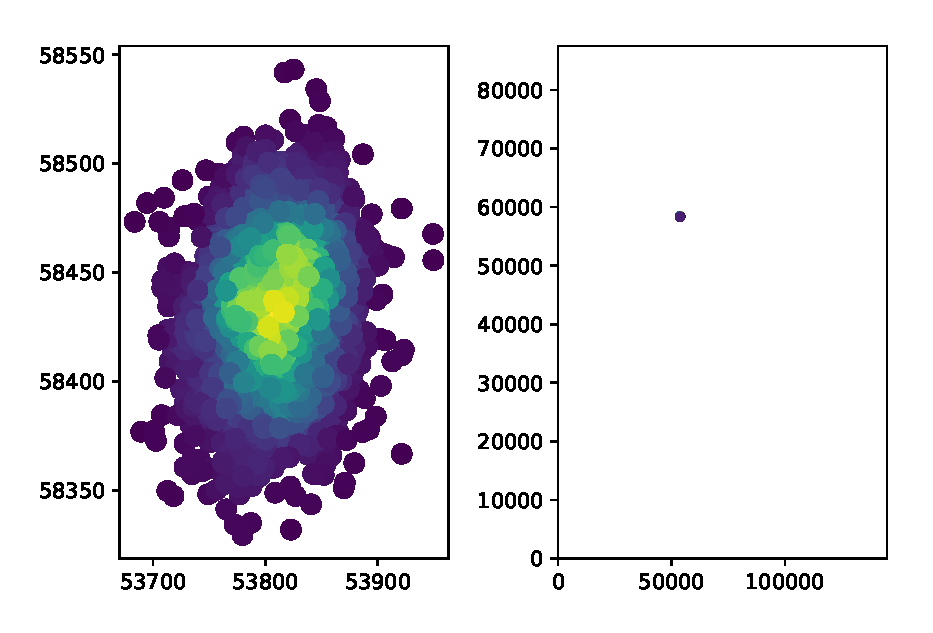
\includegraphics[width=\textwidth]{figures/dens}
		\label{fig:dens}
	\caption{Here we can see the probability density for the spatial components of the source location. The left figure is a zommed-in version of the right one. }
	\end{subfigure}
	\begin{subfigure}[b]{0.4\textwidth}
	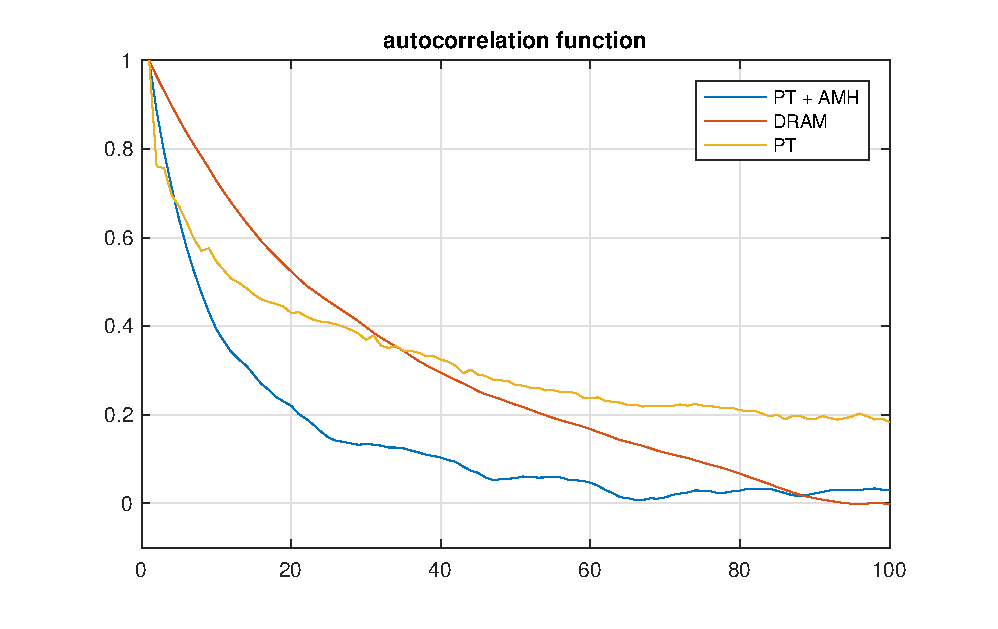
\includegraphics[width=\textwidth]{figures/acf_tanz}
		\label{fig:acf}
		\caption{Autocorrelation function for different samplers. As we can see, the most efficient sampler is the combination of parallel tempering and adaptive Metropolis. All samplers took equivalent time.  }
	\end{subfigure}
	\caption{Inversion Results}\label{fig:animals}
\end{figure}

\color{red} same as before, I have some older results on the toy problem with the KDE and some results for a toy problem using the ideal proposal (sampling for normals), but I guess including upcoming results might be better.\color{black}
\subsection{MLMCMC strategy}






\hspace*{0.3cm}
Only few works so far have dealt with Multi-level extensions of MCMC algorithms for posterior exploration in Bayesian inversion (\cite{hoang2013complexity} \cite{dodwell2015hierarchical}). Both authors address the case of parameter identification for elliptic PDEs and propose different strategies in order to build Multi-Level Metropolis-Hastings algorithms. 
%\begin{enumerate}
%	\item borrows  ideas form mlmc\dots,
%	\item introduce a hierarchy of meshes $h_\ell$, $\ell=0,\dots, L$, to which there will correspond a a posterior $\pi_\ell$ and a number of samples $N_\ell$.  
%	\item We diverge from the notation of the \cite{hoang2013complexity}, in the sense that we do not consider two different discretizations for the solution and the posterior. Moreover, we assume that we are on a finite parameter space, and as such, we don't need to introduce a mode discretization, as it is done in \cite{dodwell2015hierarchical}
%\end{enumerate}
As for multigrid methods applied to discretised (deterministic) PDEs, the key is to avoid estimating
the expected value of $Q_\ell$ directly on level $\ell$, but instead to estimate the correction with respect to the
next lower level. Since in the context of MCMC simulations, the target distribution $\pi$
depends on the discretization parameter $\ell$,
the new multilevel MCMC (MLMCMC) estimator has to be defined carefully \cite{dodwell2015hierarchical}. We will use the identity
$$\E_L=\sum_{\ell=0}^{L}\E_{\ell}[Q_\ell]-\E_{\ell-1}[Q_{\ell-1}],$$ where $Q$ is some quantity of interest and where we have used the convention that $\ell=-1$ means the expectation w.r.t the 0 measure. We define the increments $Y_\ell=Q_\ell-Q_{\ell-1}$. There are two main ideas  underlying the reduction in computational cost associated with
the multilevel estimator: \begin{itemize}
	\item Samples at level $\ell$ are cheaper to estimate
	\item The Variance of $Y_\ell$ goes to 0 as $\ell$ goes to infinity.
\end{itemize}
To guarantee the reduction in computation effort, we use the following assumptions:
\begin{assumption}\label{mlmcmc:assumptions}The following are assumed to hold:
	\begin{enumerate}
		\item $\exists \alpha>0$ such that $\Vert \uu-\uu_{h_\ell}\Vert_V\leq C_1h^{-\alpha \ell}$, where $u_\ell$ denotes the solution with discretization parameter $h_\ell$.
		\item $\exists \beta>0$ such that $\V_\ell[ Y_\ell] \leq C_2h^{-\beta \ell}$, where $u_\ell$ denotes the solution with discretization parameter $h_\ell$; $Y$ defined to be the increment as in \cite{dodwell2015hierarchical}.
		\item $\exists \gamma>0$ such that the cost $\mathcal{C}_\ell$ associated to evaluating $\pot_\ell$ behaves as $\mathcal{C}_{\ell}\leq C_3h^{-\gamma}$.
		\item We can generate samples from $\pi_\ell, \pi_{\ell-1}$ using an independent sampler MH algorithm.
	\end{enumerate}
\end{assumption}
\begin{center}
	Notice that $1$ and $3$ in Assumption \ref{mlmcmc:assumptions} are related to the PDE at hand. An algorithm that 
	\fbox{\begin{minipage}{35em}
			\begin{algorithmic}[1]
				\Function{MLMCMC}{$\{N_\ell\}_{\ell=0}^L,\{\pi_\ell\}_{\ell=0}^L,q,\theta^0$}
				\If {$\ell=0$}
				\State $\chi_{0,0}=$\texttt{Metropolis-Hastings}($N_0,\pi_0,q,\theta^0$)
				\EndIf
				\For{$\ell=1,\dots,L$}
				%\State Approximate $\pi_{\ell-1}$ by $\hat{\pi}_{\ell-1}$.
				\For {$n=1,2,\dots,N_\ell-1$}
				\State Sample $\tilde{\theta}\sim\hat{\pi}_{\ell-1} $.
				\State Set $\theta^*\sim q(\tilde{\theta})$.
				\For{$j=\ell-1,\ell$}
				\State Set $\theta_{\ell,j}^{n+1}=\theta^*$ with acceptance probability $\alpha_j$:
				$$\alpha_j(\theta_{\ell,j}^n,\theta^*)=\min \left[\frac{\pi_j(\theta^*)q(\theta_{\ell,j}^{n})\hat{\pi}_{\ell-1}(\theta_{\ell,j}^n)}{\pi_j(\theta_{\ell,j}^n)q(\theta^*)\hat{\pi}_{\ell-1}(\theta^*)},1\right].$$
				\State Set $\theta_{\ell,j}^{n+1}=\theta^n$ otherwise.
				\EndFor
				\EndFor
				\State Create chains $\chi_{\ell,\ell-1}=\{\theta_{\ell,\ell-1}^n\}_{n=0}^{N_\ell}$ and $\chi_{\ell,\ell}=\{\theta_{\ell,\ell}^n\}_{n=0}^{N_\ell}$
				\EndFor
				\State Output $\chi_{\ell,\ell},$ and $\chi_{\ell,\ell-1}$ for $\ell=0,\dots,L$.
				\EndFunction
			\end{algorithmic}
	\end{minipage}}
\end{center}
Note that in the case where we generate proposals by subsampling from the previous chain we obtain the algorithm presented in \cite{dodwell2015hierarchical}. We present some definitions that we will use throughout the rest of the paper.
\begin{definition}
	We say that at a given level $\ell$ and iteration $n$, the chain \textbf{diverged} if $\te^n_{\ell,\ell}\neq \te^n_{\ell,\ell-1}$.
\end{definition}
\subsection{On how to generate $\hat{\pi}_\ell$}
\noindent One thing that has not been discussed so far is how to choose $\hat{\pi}_{\ell}$. We now discuss some proposal generating functions for the independent sampler
\subsubsection{Ideal Proposal}
We first study the ideal, (yet no implementable for the majority of the problems), case for which we are able to do an independent sampler generating proposal from the target distribution at the previous level. That is, suppose that at each level $\ell$ , $\pi_\ell=\hat{\pi}_\ell$. Thus, given a sequence of target distributions $\{\pi_\ell\}_{\ell=1}^\infty$, we generate candidate states from $\pi_{\ell-1}$ at each iteration, i.e, we generate proposal states by $$\te^*\sim \pi_{\ell-1}.$$ Even if this \textit{oracle} algorithm is not implementable in practice for the majority of more \textit{ interesting}
problems, we can learn some of the properties that belong to the ``best case scenario" algorithm.
\begin{proposition}
	Let $\pi_{\ell-1}=\hat{\pi}_{\ell-1},$ and  let there be a $C_1$ such that $\pi_\ell\leq C_1\pi_{\ell-1}$. Then, assuming that we are on a bounded state space and that $\forall \te\in\Omega$ and $ \ell\geq0, $ we have that $\pi_\ell(\te)>0$, the following holds: \begin{enumerate}
		\item The acceptance rate $\alpha_\ell\rightarrow 1$ as $\ell\rightarrow\infty$. 
		\item The integrated autocorrelation time $\tau$ goes to 1  as $\ell\rightarrow\infty$, assuming that we can generate i.i.d samples from $\pim$.
	\end{enumerate}
%	\begin{proof}
%		Firstly, notice that for each level, the acceptance rate at the previous level $\ell-1$, is always 1 since $\hat{\pi}_{\ell-1}=\pi_{\ell-1}$. Thus:
%		$$a_{\ell-1}=\min\left[\frac{\pi_{\ell-1}(\theta^*)q(\theta_{\ell-1}^n)\pi_{\ell-1}(\theta^n)}{\pi_{\ell-1}(\theta^n)q(\theta_{\ell-1}^*)\pi_{\ell-1}(\theta^*)},1\right]=\min[1,1]=1.$$
%		This means, that the probability of diverging at any given iteration is $1-\alpha_\ell$. Thus, we have that the expected divergence at level $\ell$ is given by $$\E[1-\alpha_\ell]=1-\E[\alpha_\ell]\geq1-\frac{1}{C_1},$$
%		where Proposition \ref{prop3} was used in the inequality. Moreover, in an act of abbusive notation,  we denote $\pi_\ell,\pi_{\ell-1}$ the density of the distributions at both levels. Taking the difference of the distribution evaluated at $\te$, we obtain \begin{align}
%		|\pim-\pil|&=\left\vert \frac{e^{-\potm}}{Z_\ell}-\frac{e^{-\potl}}{Z_{\ell-1}}\right\vert \leq \left\vert \frac{e^{-\potl}}{Z_{\ell}} -\frac{e^{-\potl}}{Z_{\ell-1}}\right\vert +\left \vert \frac{e^{-\potm}}{\zm}-\frac{e^{-\potl}}{\zm} \right \vert \nonumber \\
%		&= \lv \frac{1}{\zm}\rv \lv e^{-\potm}-e^{-\potl}\rv+\lv \frac{e^{-\potl}}{\zl}\rv\lv1-\frac{\zl}{\zm}\rv \nonumber \\
%		&\leq \lno \uu_\ell-\uu_{\ell-1}\rno_X+\lv \frac{e^{-\potl}}{\zl}\rv \lv \frac{\zm-\zl}{\zl\zm}\rv \nonumber \\
%		&\leq \lv \frac{1}{\zl}\rv \left[  c_{\te} h^{\alpha\ell}+\frac{e^{\Phi(r)}}{|\zl\zm|}\lv\zm-\zl\rv \right].
%		\end{align}
%		Now, notice that $$\lv \zm-\zm\rv =\lv \int_\Omega e^{-\potm}-e^{-\potl}d\pi^0\rv\leq  \int_\Omega \lv e^{-\potm}-e^{-\potl}\rv d\pi^0,$$
%		Thus, we have that 
%		$$ \int_\Omega \lv e^{-\potm}-e^{-\potl}\rv d\pi^0\leq \int_\Omega \lv \uu_\ell -\uu_{\ell-1}\rv d\pi^0\leq C_{\te} h^{\alpha \ell }$$
%		Finally since $(1/C_1)\leq \pil/\pim$, we have that $$\left(1-\frac{1}{C_\ell}\right)\vert\pil\vert=\vert(1-\frac{1}{C_\ell})\pil\vert    \leq\vert \pil\left(1-\frac{\pim}{\pil}\right)\vert\leq  K_\ell(\te)h^{\alpha\ell},$$
%		and as such, $\E[\text{divergence}]\rightarrow 0$ as $\ell\rightarrow\infty$.
%		The second part is evident; under the assumption that we can generate iid samples from $\pi_{\ell-1}$, and since the acceptance rate tends to 1, then the autocorrelation of the samples at level $\ell$ will become 0. 
%	\end{proof}
%	
	
\end{proposition}	
\subsubsection{Sampling From the Prior}
\color{red}there is a result that quantifies the conv. rate for ind. sampler based on bounds of the lielihhod, i'll include it soon \color{black}
\subsubsection{KDE approximation}
One possible way of generating $\hat{\pi}_{\ell-1}$ is to create a KDE based on the samples obtained at the previous level. 
\subsubsection{Laplace's Approximation}
Alternatively , we can use Laplace's approximation in order to compute $\hat{\pi}_{\ell-1}$ under the assumptions that (i) it is a smooth function in $\Omega$ and (ii) that the distribution is well peaked. Under these assumptions, we have that, denoting $q_{\ell-1}(\te)=\hat{\pi}_{\ell-1}$ and  omitting the dependence on the level for notational clarity, the Taylor expansion of $q(\te)$ around is maximum a posteriori (MAP) $\te^{MAP}$ is given by 
\begin{align}
q(\te)&=q(\te')+(\te-\te^{MAP})^T\del q(\te)+\frac{1}{2}(\te-\te^{MAP})^TH(\te-\te^{MAP}) + \mathcal{O}((\te-\te^{MAP})^3) \nonumber,\\
&=q(\te')+\frac{1}{2}(\te-\te^{MAP})^TH(\te-\te^{MAP}) + \mathcal{O}((\te-\te^{MAP})^3), \ \ \text {since $\del q(\te^{MAP})=0$}\nonumber,\\
&\approx C-\frac{1}{2}(\te-\te^{MAP})^TH(\te-\te^{MAP}),
\end{align}
%	 	which can be interpreted as the logarithm of a normal distribution with variance $H$ (the Hessian) with mean $\te^{MAP}$. Moreover, it can be shown  \cite{schillings2018} that \begin{align}
%	 	d^2_{Hell}(\pi,\hat{\pi})\in \mathcal{O}
%	 	\end{align}  
Despite being an interesting approach and having some desirable properties (see \cite{schillings2018}), this approach has two main drawbacks. The first one is the lack of generality, as it is not always the case that a posterior has a unique maximizer. The second one is the computational challenge of computing the Hessian. This however, can be approximated and computed "in line" if an optimization algorithm is used to find the MAP. 
\subsubsection{Optimization of a Parametric Family}
An additional approach to computing $\hat{\pi}_{\ell-1}$ is as based on the minimization of the Hellinger distance between $\pi_{\ell-1}$ and $\hat{\pi}_{\ell-1}$. Formally, we seek to approximate ${\pi}_{\ell-1}$ using a parametric family of distributions with density  $f(\te;\gamma)$, where $\gamma$ is given by \begin{align}
\gamma^*=\min_{\gamma\in \Gamma}\int_\Omega \frac{1}{2}\left(\sqrt{\hat{\pi}_{\ell-1}}-\sqrt{f(\te;\gamma)}\right)^2d\gamma +\frac{\alpha}{2}R(\gamma),
\end{align}
where $R$ is a regularizer with regularization term $\alpha$.  Notice that the previous integral can be rewritten in terms of an expectation with respect to the samples of the previous  chain $\chi_{\ell-1,\ell-1}$ as \begin{align}
\E_{\pi_{\ell-1}}\left[ \left(\sqrt{{\pi}_{\ell-1}}-\sqrt{f(\te;\gamma)}\right)^2\frac{1}{{\pi}_{\ell-1}}	\right],
\end{align}
thus, the optimization problem can be read as find $\gamma^*$ such that
\begin{align}
\gamma^*=\min_{\gamma\in \Gamma}\ \ \E_{\pi_{\ell-1}}\left[ \left(\sqrt{{\pi}_{\ell-1}}-\sqrt{f(\te;\gamma)}\right)^2\frac{1}{{\pi}_{\ell-1}}	\right]+\frac{\alpha}{2}R(\gamma).
\end{align}
This expectation can in turn be approximated with error $N_\ell^{1/2}$ by 
\begin{align}
\approx\frac{1}{N_\ell}\sum_{i=1}^{N_\ell}\left[\left(\sqrt{{\pi}_{\ell-1}(\te^i)}-\sqrt{f(\te^i;\gamma)}\right)^2 {\pi}^{-1}_{\ell-1}(\te ^i )\right]+\frac{\alpha}{2}R(\gamma).
\end{align}
Moreover, note that it is possible to save the values of the un-normalized posterior $\pi_{\ell-1}$ at the previous level,  and as such, this optimization algorithm should represent a  lower cost with respect to the solution of the PDE. Moreover, note that each approximation can be improved at the next level, given that each chain is evaluated twice in the algorithm.  Alternatively, a similar approach can be proposed minimizing the Kullback-Lieber divergence.

%\noindent Notice that when using SEM (with $p\geq 1)$ with a regular grid, the discretization error is dominated by the time-error. Moreover, from the CFL condition we have that $h=\mathcal{O}(\dt)$, and as such, the ``worst case scenario" (for long time integration) we have that $\alpha =2$. A similar argument holds for assumption $(ii)$. Assumption $(iii) $ is shown in \dots, which is an adaptation for our case of proposition 5 in \cite{hoang2013complexity}. Assumption $(iv)$ follows trivially. 

